\documentclass[11pt,a4paper]{article}
\usepackage[T1]{fontenc}
\usepackage[utf8]{inputenc}
\usepackage{lmodern}
\usepackage{textcomp}
\usepackage[left=1.8cm,right=1.8cm,top=3.0cm,bottom=2.2cm,headheight=36pt,headsep=12pt]{geometry}
\usepackage{multicol}
\usepackage{xcolor}
\usepackage{fancyhdr}\usepackage{tikz}
\usepackage{graphicx}
\usepackage{array}
\usepackage{amsmath,amssymb}
\usepackage{setspace}
\usepackage{longtable}
\graphicspath{{../}}
\definecolor{ygreen}{RGB}{46,139,87}\definecolor{dgreen}{RGB}{28,90,56}
\renewcommand{\normalsize}{\fontsize{10.9}{13.4}\selectfont}
\renewcommand{\familydefault}{\rmdefault}
\setlength{\parindent}{0pt}
\setlength{\columnsep}{0.8cm}
\setlength{\columnseprule}{0.4pt}
\setlength{\multicolsep}{3pt plus 1pt minus 1pt}
\renewcommand{\textsubscript}[1]{\ensuremath{_{\text{\fontsize{8}{8}\selectfont #1}}}}
\renewcommand{\textsuperscript}[1]{\ensuremath{^{\text{\fontsize{8}{8}\selectfont #1}}}}
\newcommand{\qn}[1]{\textbf{\fontsize{11.5}{13}\selectfont #1}}
\newcommand{\qsep}{\par\vspace{13pt}}
\newcommand{\fwrule}{\par\vspace{5pt}\noindent\rule{\linewidth}{1.4pt}\par\vspace{7pt}}
\newsavebox{\fitb}
\newcommand{\fitbox}[1]{\sbox{\fitb}{#1}\ifdim\wd\fitb>\linewidth\resizebox{\linewidth}{!}{\usebox{\fitb}}\else\usebox{\fitb}\fi}
\newcommand{\diqqat}[1]{\par\smallskip\noindent\textbf{Diqqat!} #1\par\medskip}
\newcommand{\javob}{\par\nopagebreak[4]\smallskip\noindent\textbf{Javob:} \rule[-2pt]{7.5cm}{0.4pt}\par\smallskip\noindent\textbf{Diqqat!} Javobingizni javoblar varaqasiga ko`chirib yozing.\par\medskip}
\pagestyle{fancy}
\fancyhf{}
\renewcommand{\headrulewidth}{1.6pt}\renewcommand{\headrule}{{\color{ygreen}\hrule height 1.6pt width\headwidth}}
\newcommand{\hdrlogo}{
\begin{tikzpicture}[baseline=0pt]\fill[ygreen,rounded corners=3pt] (0,0) rectangle (0.95,0.95);\node[white,font=\fontsize{24}{26}\bfseries\selectfont] at (0.475,0.47){K};\node[anchor=west,font=\fontsize{16}{18}\bfseries\selectfont,text=dgreen] at (1.15,0.66){KIMYO};\node[anchor=west,font=\footnotesize\scshape,text=gray] at (1.15,0.2){Milliy sertifikat\ \ 2026};\end{tikzpicture}}
\newcommand{\hdrpill}[1]{\begin{tikzpicture}[baseline=0pt]\node[fill=ygreen,text=white,rounded corners=8pt,inner xsep=10pt,inner ysep=5pt,font=\fontsize{13}{15}\bfseries\selectfont] at (0,0.475){#1};\end{tikzpicture}}
\fancyhead[L]{\hdrlogo}
\fancyhead[R]{\hdrpill{4-variant}}

\fancyfoot[C]{\thepage}
\fancypagestyle{first}{\fancyhf{}\renewcommand{\headrulewidth}{1.6pt}\renewcommand{\headrule}{{\color{ygreen}\hrule height 1.6pt width\headwidth}}\fancyhead[L]{\hdrlogo}\fancyhead[R]{\hdrpill{4-variant}}\fancyfoot[C]{\thepage}}
\begin{document}
\normalsize
\thispagestyle{first}
\noindent\textit{Davriy jadvaldan foydalanish mumkin.}
\par\smallskip
\begin{multicols}{2}
\noindent\qn{1.} 17-tartib raqamli elementning barcha elektronlaridan nechtasining spin kvant soni m\_s = +$\frac{1}{2}$ ga teng (Hund qoidasi bo`yicha to`ldirilgan holat)?

\noindent A)~\textsl{9} \hfill B)~\textsl{10} \hfill C)~\textsl{8} \hfill D)~\textsl{11}\par
\qsep
\noindent\qn{2.} Cr (Ar = 52) ning oksidida kislorodning massa ulushi 23,5\% ga teng. Oksidning \textbf{formulasini aniqlang.}

\noindent A)~\textsl{Cr\textsubscript{2}O\textsubscript{3}} \hfill B)~\textsl{CrO\textsubscript{3}} \hfill C)~\textsl{Cr\textsubscript{2}O} \hfill D)~\textsl{CrO}\par
\qsep
\noindent\qn{3.} Qaysi juftliklarda reaksiya boradi? 1) Al va CuSO\textsubscript{4}; 2) Ag va CuSO\textsubscript{4}; 3) Cu va ZnSO\textsubscript{4}; 4) Cu va AgNO\textsubscript{3}

\noindent A)~\textsl{1, 4} \hfill B)~\textsl{1, 2} \hfill C)~\textsl{2, 3} \hfill D)~\textsl{3, 4}\par
\qsep
\noindent\qn{4.} Mo`l kislota bilan Zn ning turli massalari ta'sirlashganda ajralgan H\textsubscript{2} hajmi grafikda keltirilgan (n.sh.).
\begin{center}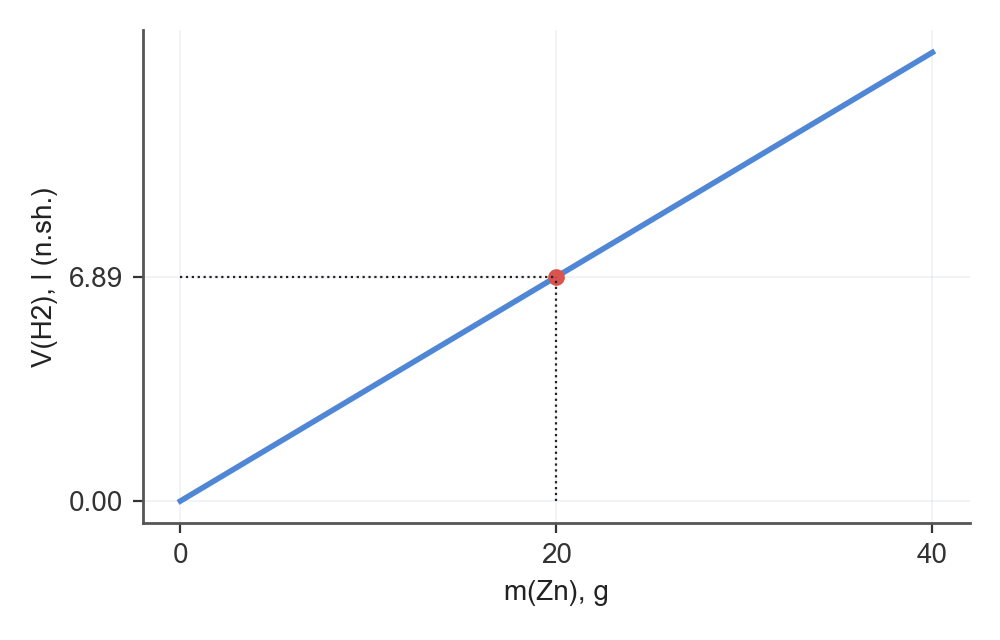
\includegraphics[width=0.86\linewidth]{rasmlar/gen/li_v04_0.png}\end{center}
Zn ning molyar massasini (g/mol) grafikdan \textbf{aniqlang.}

\noindent A)~\textsl{130} \hfill B)~\textsl{65} \hfill C)~\textsl{32,5} \hfill D)~\textsl{87,4}\par
\qsep
\noindent\qn{5.} 120 g 8\% li tuz eritmasidan suv bug`latilganda tuzning massa ulushi 4/3 marta ortdi. Bug`latilgan suv \textbf{massasini (g) toping.}

\noindent A)~\textsl{30} \hfill B)~\textsl{60} \hfill C)~\textsl{90} \hfill D)~\textsl{160}\par
\qsep
\noindent\qn{6.} Faqat oksidlovchi bo`la oladigan \textbf{ionlarni aniqlang}: 1) S\textsuperscript{2$-$}; 2) Fe\textsuperscript{2+}; 3) Al\textsuperscript{3+}; 4) Na\textsuperscript{+}

\noindent A)~\textsl{1, 2, 3} \hfill B)~\textsl{1, 3} \hfill C)~\textsl{3, 4} \hfill D)~\textsl{1, 4}\par
\qsep
\noindent\qn{7.} Tuzning eruvchanligi yuqori haroratda 100 g, past haroratda 30 g (100 g suvda). Yuqori haroratda to`yingan 200 g eritma past haroratgacha sovitilsa, necha gramm tuz cho`kmaga tushadi?

\noindent A)~\textsl{70} \hfill B)~\textsl{100} \hfill C)~\textsl{30} \hfill D)~\textsl{140}\par
\qsep
\noindent\qn{8.} A moddaning parchalanish reaksiyasida konsentratsiyaning vaqt bo`yicha o`zgarishi jadvalda berilgan:
\begin{center}
\renewcommand{\arraystretch}{1.15}
\fitbox{\begin{tabular}{|c|c|}\hline
\textbf{t, min} & \textbf{c, mol/l} \\ \hline
0 & 1,6 \\ \hline
2 & 1,44 \\ \hline
4 & 1,28 \\ \hline
6 & 1,12 \\ \hline
\end{tabular}}
\end{center}
2-minutdan 6-minutgacha o`rtacha tezlikni mol/(l$\cdot$min) \textbf{hisoblang.}

\noindent A)~\textsl{0,16} \hfill B)~\textsl{0,04} \hfill C)~\textsl{0,08} \hfill D)~\textsl{0,32}\par
\qsep
\noindent\qn{9.} 2SO\textsubscript{3} $\rightleftarrows$ 2SO\textsubscript{2} + O\textsubscript{2} reaksiyasi doimiy harorat va bosimda olib borildi; boshlang`ich modda qisman o`zgargach gazlar hajmi 5/4 marta ortdi. Boshlang`ich modda necha foizi \textbf{o`zgarganini aniqlang.}

\noindent A)~\textsl{25} \hfill B)~\textsl{50} \hfill C)~\textsl{60} \hfill D)~\textsl{100}\par
\qsep
\noindent\qn{10.} CO + Cl\textsubscript{2} $\rightleftarrows$ COCl\textsubscript{2} reaksiyasi 5 l hajmli idishda o`tkazildi. Ma'lumotlar jadvalda berilgan:
\begin{center}
\renewcommand{\arraystretch}{1.15}
\fitbox{\begin{tabular}{|c|c|c|c|}\hline
\textbf{Modda} & \textbf{CO} & \textbf{Cl\textsubscript{2}} & \textbf{COCl\textsubscript{2}} \\ \hline
Boshlang`ich, mol & 3 & 4 & 0 \\ \hline
Muvozanatda, mol & --- & --- & 1,5 \\ \hline
\end{tabular}}
\end{center}
Muvozanat \textbf{konstantasini (K) hisoblang.}

\noindent A)~\textsl{4} \hfill B)~\textsl{1} \hfill C)~\textsl{2} \hfill D)~\textsl{10}\par
\qsep
\noindent\qn{11.} 2SO\textsubscript{2} + O\textsubscript{2} $\rightleftarrows$ 2SO\textsubscript{3} + Q muvozanatni o`ngga siljitadigan \textbf{o`zgarishlarni toping}: 1) bosimni pasaytirish; 2) bosimni oshirish; 3) haroratni pasaytirish; 4) haroratni oshirish.

\noindent A)~\textsl{2, 3, 4} \hfill B)~\textsl{4} \hfill C)~\textsl{1, 2, 3} \hfill D)~\textsl{2, 3}\par
\qsep
\noindent\qn{12.} NaCl eritmasi inert elektrodlar bilan 5 A tok kuchi bilan 965 s elektroliz qilindi. Ajralgan gazlar aralashmasi yondirilib, hosil bo`lgan gaz 400 g suvda eritildi. Olingan kislota eritmasining massa \textbf{ulushini (\%) aniqlang.}

\noindent A)~\textsl{0,23} \hfill B)~\textsl{0,45} \hfill C)~\textsl{0,46} \hfill D)~\textsl{0,91}\par
\qsep
\noindent\qn{13.} 2NO + O\textsubscript{2} $\to$ 2NO\textsubscript{2} reaksiyasida (v = k$\cdot$[NO]\textsuperscript{2}$\cdot$[O\textsubscript{2}]) harorat 40 \textdegree{}C ga oshirildi ($\gamma$ = 2), shu bilan birga NO konsentratsiyasi 2 marta kamaytirildi. Reaksiya tezligi qanday o`zgaradi (necha marta ortadi/kamayadi)? Tezlikning yangi/eski \textbf{nisbatini toping.}

\noindent A)~\textsl{8} \hfill B)~\textsl{2} \hfill C)~\textsl{16} \hfill D)~\textsl{4}\par
\qsep
\noindent\qn{14.} Probirkalardagi eritmalar: Na\textsubscript{2}SO\textsubscript{4}, Na\textsubscript{2}CO\textsubscript{3}, NaCl ni alohida probirkalarda ajratish uchun qaysi reagent(lar) yetarli? 1) HCl va fenolftalein; 2) BaCl\textsubscript{2} va fenolftalein; 3) HCl va lakmus; 4) lakmus va fenolftalein

\noindent A)~\textsl{2} \hfill B)~\textsl{4} \hfill C)~\textsl{1, 3} \hfill D)~\textsl{2, 4}\par
\qsep
\noindent\qn{15.} Zn(NO\textsubscript{3})\textsubscript{2} qizdirilganda qanday moddalar hosil bo`ladi?

\noindent\begin{tabular}{@{}p{0.47\linewidth}@{}p{0.47\linewidth}@{}}
A)~\textsl{NaNO\textsubscript{2} va O\textsubscript{2}} & B)~\textsl{CuO, NO\textsubscript{2} va O\textsubscript{2}} \\
C)~\textsl{ZnO, NO\textsubscript{2} va O\textsubscript{2}} & D)~\textsl{Ag, NO\textsubscript{2} va O\textsubscript{2}} \\
\end{tabular}\par
\qsep
\noindent\qn{16.} Qaysi juftliklar o`zaro reaksiyaga kirishadi? 1) Cu va HCl; 2) NaCl va HNO\textsubscript{3}; 3) ZnO va HCl; 4) Ag va H\textsubscript{2}SO\textsubscript{4}(suyult.)

\noindent A)~\textsl{1, 2} \hfill B)~\textsl{2, 3} \hfill C)~\textsl{3} \hfill D)~\textsl{2, 4}\par
\qsep
\noindent\qn{17.} Oksidlanish darajasi +2 bo`lgan noma'lum \textit{X} metallning oksidi 10\% li sulfat kislota eritmasining stexiometrik miqdorida to`liq eritildi. Hosil bo`lgan tuzning massa ulushi 11,76\% ga teng bo`ldi. \textit{X} \textbf{ni aniqlang.}

\noindent A)~\textsl{Mg} \hfill B)~\textsl{Ni} \hfill C)~\textsl{Cu} \hfill D)~\textsl{Ca}\par
\qsep
\noindent\qn{18.} Na\textsubscript{2}HPO\textsubscript{4} tuzining kristallogidratida suvning massa ulushi 60,3\% ni tashkil etadi. Kristallogidrat formulasidagi suv molekulalari \textbf{sonini (n) toping.}

\noindent A)~\textsl{10} \hfill B)~\textsl{24} \hfill C)~\textsl{14} \hfill D)~\textsl{12}\par
\qsep
\noindent\qn{19.} 0,4 mol NH\textsubscript{4}Cl ning mo`l NaOH eritmasi bilan qizdirilishidan ajralgan ammiak 200 g suvga to`liq yuttirildi. Reagent (NaOH) eritmasining massa ulushi 20\% va zichligi 1,3 g/ml; u mo`l miqdorda olingan. Hosil bo`lgan eritmadagi ammiakning massa \textbf{ulushini (\%) toping.}

\noindent A)~\textsl{3,4} \hfill B)~\textsl{3,29} \hfill C)~\textsl{7,1} \hfill D)~\textsl{6,58}\par
\qsep
\noindent\qn{20.} Rasmda $\alpha$-aminokislotaning tuzilish formulasi berilgan.
\begin{center}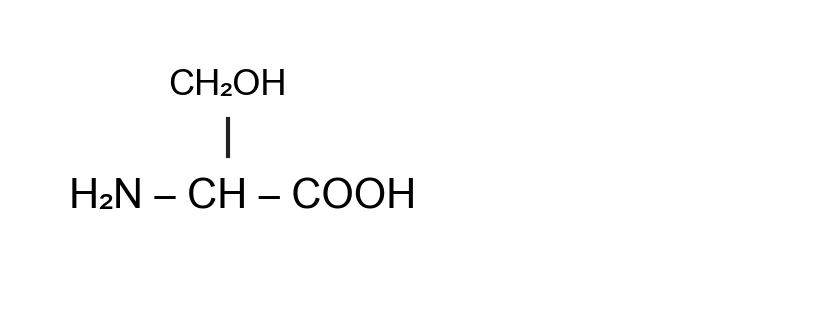
\includegraphics[width=0.86\linewidth]{rasmlar/gen/aa_999520.png}\end{center}
Aminokislotaning \textbf{nomini toping.}

\noindent A)~\textsl{serin} \hfill B)~\textsl{alanin} \hfill C)~\textsl{glitsin} \hfill D)~\textsl{valin}\par
\qsep
\noindent\qn{21.} Alken, alkadiyen va alkinlar haqida qaysi fikrlar to`g`ri? 1) Alkinlar uchun umumiy formula CnH\textsubscript{2}n+2; 2) Etilen bromli suvni rangsizlantiradi; 3) Asetilenni Kucherov reaksiyasi bilan sirka aldegidiga aylantirish mumkin; 4) Asetilen Ag\textsubscript{2}O ning ammiakli eritmasi bilan cho`kma beradi (butin-2 beradi)

\noindent A)~\textsl{3} \hfill B)~\textsl{1, 2, 4} \hfill C)~\textsl{2, 3} \hfill D)~\textsl{2, 4}\par
\qsep
\noindent\qn{22.} Karbon kislotalar haqida qaysi fikrlar to`g`ri? 1) Benzoy kislota Na\textsubscript{2}CO\textsubscript{3} bilan reaksiyaga kirishmaydi; 2) Qattiq suvda sovun yaxshi ko`piklanadi; 3) Sirka angidrid ikki molekula sirka kislotadan suv chiqib hosil bo`ladi; 4) Karboksil guruh karbonil va gidroksil guruhlardan iborat

\noindent A)~\textsl{2} \hfill B)~\textsl{3} \hfill C)~\textsl{3, 4} \hfill D)~\textsl{4}\par
\qsep
\noindent\qn{23.} Formaldegid va etanal aralashmasi (14 g) mo`l ammiakli kumush oksid eritmasi bilan qizdirilganda 97,2 g kumush ajraldi. Aralashmadagi formaldegidning \textbf{massasini (g) aniqlang.}

\noindent A)~\textsl{11} \hfill B)~\textsl{3} \hfill C)~\textsl{6} \hfill D)~\textsl{7}\par
\qsep
\noindent\qn{24.} Etilformiat va propilatsetat aralashmasi (60,2 g) mo`l NaOH eritmasi bilan to`liq gidrolizlandi. Aralashmaning mol miqdori 0,7 mol. Reagent (NaOH) eritmasining massa ulushi 36\% va zichligi 1,3 g/ml; u mo`l miqdorda olingan. Hosil bo`lgan tuzlar \textbf{massasini (g) aniqlang.}

\noindent A)~\textsl{103,6} \hfill B)~\textsl{51,8} \hfill C)~\textsl{60,2} \hfill D)~\textsl{52,5}\par
\qsep
\noindent\qn{25.} 324 g kraxmal gidrolizlanib (unum 80\%) glukoza olindi, glukoza esa spirtli bijg`ishga uchradi (unum 50\%). Barcha reaksiyalar 1 atm bosimda olib borildi. Hosil bo`lgan etanol \textbf{massasini (g) toping.}

\noindent A)~\textsl{36,8} \hfill B)~\textsl{147,2} \hfill C)~\textsl{184} \hfill D)~\textsl{73,6}\par
\qsep
\noindent\qn{26.} 256 g CaC\textsubscript{2} dan quyidagi sxema bo`yicha 26,98 g anilin olindi: CaC\textsubscript{2} $\to$ C\textsubscript{2}H\textsubscript{2} $\to$ C\textsubscript{6}H\textsubscript{6} $\to$ C\textsubscript{6}H\textsubscript{5}NO\textsubscript{2} $\to$ C\textsubscript{6}H\textsubscript{5}NH\textsubscript{2}. Dastlabki 3 bosqichning unumi ketma-ket 40\%, 80\%, 85\% ga teng. Barcha reaksiyalar 1 atm bosimda olib borildi. Oxirgi bosqichning \textbf{unumini (\%) aniqlang.}

\noindent A)~\textsl{40} \hfill B)~\textsl{20} \hfill C)~\textsl{64} \hfill D)~\textsl{80}\par
\qsep
\noindent\qn{27.} CH\textsubscript{4} dan quyidagi sxema bo`yicha 15,12 g etilen olindi: CH\textsubscript{4} $\to$ CH\textsubscript{3}Cl $\to$ C\textsubscript{2}H\textsubscript{6} $\to$ C\textsubscript{2}H\textsubscript{4}. Bosqichlarning unumi ketma-ket 90\%, 40\%, 75\% ni tashkil qiladi. Sarflangan CH\textsubscript{4} hajmi (l, n.sh.) \textbf{ni aniqlang.}

\noindent A)~\textsl{179,2} \hfill B)~\textsl{44,8} \hfill C)~\textsl{89,6} \hfill D)~\textsl{80,64}\par
\qsep
\noindent\qn{28.} C\textsubscript{6}H\textsubscript{6} dan quyidagi sxema bo`yicha 83,78 g 2,4,6-tribromfenol olindi: C\textsubscript{6}H\textsubscript{6} $\to$ C\textsubscript{6}H\textsubscript{5}Cl $\to$ C\textsubscript{6}H\textsubscript{5}OH $\to$ C\textsubscript{6}H\textsubscript{2}Br\textsubscript{3}OH. Bosqichlarning unumi ketma-ket 75\%, 90\%, 75\% ni tashkil qiladi. Sarflangan C\textsubscript{6}H\textsubscript{6} massasi (g) \textbf{ni aniqlang.}

\noindent A)~\textsl{78} \hfill B)~\textsl{19,5} \hfill C)~\textsl{29,25} \hfill D)~\textsl{39}\par
\qsep
\noindent\qn{29.} 184 g C\textsubscript{2}H\textsubscript{5}OH dan quyidagi sxema bo`yicha etilenglikol olindi: C\textsubscript{2}H\textsubscript{5}OH $\to$ C\textsubscript{2}H\textsubscript{4} $\to$ HOCH\textsubscript{2}--CH\textsubscript{2}OH. Bosqichlarning unumi ketma-ket 60\%, 90\% ni tashkil qiladi. Olingan etilenglikol \textbf{massasini (g) aniqlang.}

\noindent A)~\textsl{267,84} \hfill B)~\textsl{66,96} \hfill C)~\textsl{148,8} \hfill D)~\textsl{133,92}\par
\qsep
\noindent\qn{30.} Kimyo laboratoriyasida ishlash qoidalari haqida qaysi fikrlar to`g`ri? 1) Reaktivlarni tatib ko`rish mumkin; 2) Kuygan joy ko`p suv bilan yuviladi; 3) Ishqor teriga tushsa, qo`l suv bilan yuviladi; 4) Konsentrlangan kislotani suvga ohista, aralashtirib quyiladi

\noindent A)~\textsl{1, 4} \hfill B)~\textsl{2, 3, 4} \hfill C)~\textsl{2, 3} \hfill D)~\textsl{1, 3, 4}\par
\qsep
\noindent\qn{31.} Raqamlangan (1--4) probirkalarda HCl, Na\textsubscript{2}S, NaOH, Pb(NO\textsubscript{3})\textsubscript{2} eritmalari tartibsiz holda berilgan. Quyidagi kuzatuvlar asosida moddalarni probirka raqami bilan moslang. 1- va 4-probirkalardagi eritmalar aralashtirilganda oq cho`kma tushadi (mo`l ishqorda eriydi). 2- va 3-probirkalardagi eritmalar aralashtirilganda chirigan tuxum hidli gaz ajraladi. 3- va 4-probirkalardagi eritmalar aralashtirilganda bir-birini neytrallaydi.
\noindent A)~\textsl{1-Pb(NO\textsubscript{3})\textsubscript{2}, 2-Na\textsubscript{2}S, 3-HCl, 4-NaOH}\par
\noindent B)~\textsl{1-Pb(NO\textsubscript{3})\textsubscript{2}, 2-HCl, 3-Na\textsubscript{2}S, 4-NaOH}\par
\noindent C)~\textsl{1-NaOH, 2-Na\textsubscript{2}S, 3-HCl, 4-Pb(NO\textsubscript{3})\textsubscript{2}}\par
\noindent D)~\textsl{1-Na\textsubscript{2}S, 2-Pb(NO\textsubscript{3})\textsubscript{2}, 3-HCl, 4-NaOH}\par
\qsep
\noindent\qn{32.} Rasmdagi tajribada efirlanish reaksiyasida konsentrlangan H\textsubscript{2}SO\textsubscript{4} qanday vazifani bajaradi?
\begin{center}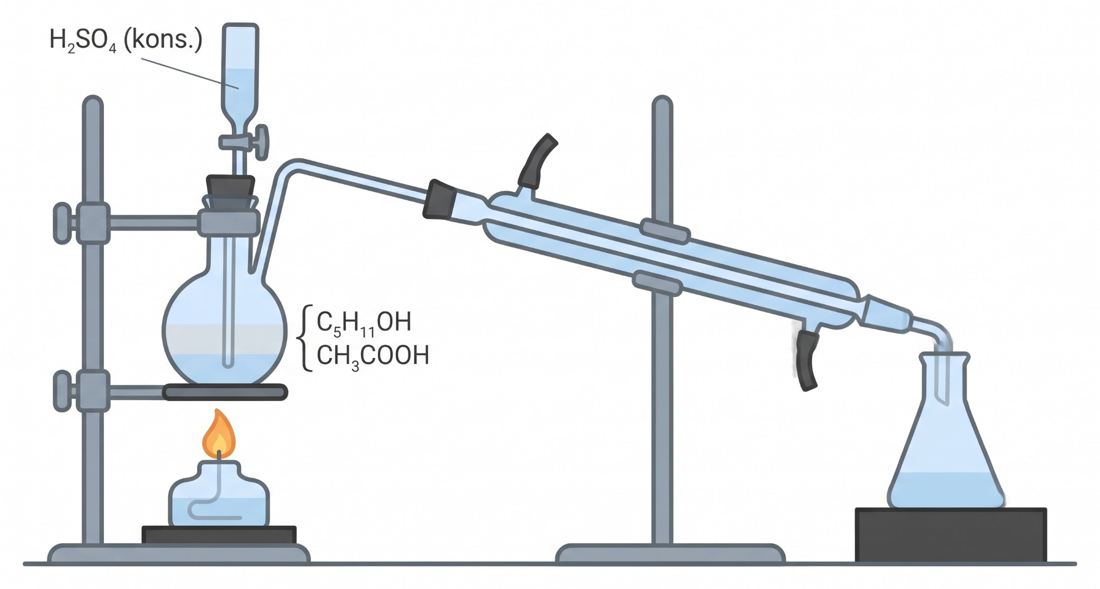
\includegraphics[width=0.86\linewidth]{rasmlar/darslik/d_efir.png}\end{center}
\noindent A)~\textsl{reaksiya mahsuloti}\par
\noindent B)~\textsl{katalizator va suv tortuvchi}\par
\noindent C)~\textsl{oksidlovchi}\par
\noindent D)~\textsl{faqat erituvchi   ---}\par
\qsep
\end{multicols}
\medskip
\noindent\setlength{\fboxsep}{0pt}\fbox{\begin{tabular}{p{0.74\linewidth}|p{0.2\linewidth}}
\parbox[t]{0.72\linewidth}{\vspace{3pt}\textbf{Topshiriqlar (33--35) va javob variant (A--F)larini o`zaro to`g`ri moslashtiring.} 100 g CuSO\textsubscript{4}$\cdot$5H\textsubscript{2}O suvda eritilib, eritmaga mo`l NaOH eritmasi qo`shildi, hosil bo`lgan cho`kma ajratilib, doimiy massagacha qizdirildi.
\vspace{3pt}} & \parbox[t]{0.19\linewidth}{\vspace{3pt}A~\textsl{85,2}\\[3pt]
B~\textsl{39,2}\\[3pt]
C~\textsl{16}\\[3pt]
D~\textsl{19,6}\\[3pt]
E~\textsl{32}\\[3pt]
F~\textsl{56,8}}\\ \hline
\parbox[t]{0.72\linewidth}{\vspace{2pt}\textbf{33. Cho`kmaning massasini (g) aniqlang.}\vspace{2pt}} & \\ \hline
\parbox[t]{0.72\linewidth}{\vspace{2pt}\textbf{34. Qizdirishdan so`ng qolgan qattiq moddaning massasini (g) toping.}\vspace{2pt}} & \\ \hline
\parbox[t]{0.72\linewidth}{\vspace{2pt}\textbf{35. Cho`kma hosil bo`lgandan keyin eritmada qolgan natriy sulfat massasini (g) hisoblang.}\vspace{2pt}} & 
\end{tabular}}
\par\bigskip
\noindent\qn{36.} 10\% li va 5\% li tuz eritmalari massalar nisbati 2 : 3 bo`lgan holda aralashtirildi. Tajriba 20 daqiqa davom etdi. Hosil bo`lgan eritmaning massa \textbf{ulushini (\%) hisoblang.}
\javob\qsep
\noindent\qn{37.} 200 g 10\% li CuSO\textsubscript{4} eritmasiga m g CuSO\textsubscript{4}$\cdot$5H\textsubscript{2}O eritildi, natijada tuzning massa ulushi 20,8\% ga yetdi. Tajriba 10 daqiqa davom etdi. m \textbf{ni (g) toping.}
\javob\qsep
\noindent\qn{38.} Al, Fe va Cu dan iborat aralashma mo`l NaOH eritmasi bilan ta'sirlashganda 6,72 l (n.sh.) vodorod ajraldi; xuddi shunday massadagi aralashma mo`l HCl bilan ta'sirlashganda 11,2 l (n.sh.) vodorod ajraldi, erimay qolgan qoldiq (mis) massasi 6,4 g. Aralashmaning zichligi 5,2 g/sm\textsuperscript{3} ga teng. Aralashmaning dastlabki \textbf{massasini (g) toping.}
\javob\qsep
\noindent\qn{39.} Noma'lum alkenning 4,2 g miqdori mo`l brom suvi bilan to`liq reaksiyaga kirishganda 16 g brom sarflandi. Xuddi shu alkenning 3/4 qismi gidratlanib spirtga aylantirildi, hosil bo`lgan spirt natriy bilan ta'sirlashtirildi. Reagent (brom suvi) eritmasining massa ulushi 10\% va zichligi 1,3 g/ml; u mo`l miqdorda olingan. Ajralgan vodorod \textbf{hajmini (l, n.sh.) toping.}
\javob\qsep
\noindent\qn{40.} 22,4 l (n.sh.) atsetilen Kucherov reaksiyasi bo`yicha gidratlandi (unum 1/2); hosil bo`lgan aldegidning 3/5 qismi ammiakli kumush oksid eritmasi bilan qizdirildi. Barcha reaksiyalar 1,5 atm bosimda olib borildi. Ajralgan kumush \textbf{massasini (g) hisoblang.}
\javob\qsep
\par\bigskip\begin{center}\textbf{\fontsize{13}{15}\selectfont YOZMA ISH}\end{center}
\noindent\qn{41.} \textbf{Topshiriqni bajarish jarayonida barcha reaksiya tenglamalarini yozing. Miqdoriy va arifmetik hisoblashlarni (unga asos bo`lgan usul yoki formulani ko`rsatgan holda) uzviy ketma-ketlikda bajaring.}\par\smallskip
Cu(NO\textsubscript{3})\textsubscript{2} va NaNO\textsubscript{3} dan iborat 44,25 g aralashma doimiy massagacha qizdirildi. Ajralgan gazlar aralashmasi sovitilib, 300 g suvga yuborildi Qattiq qoldiq suvga tushirilganda NaNO\textsubscript{2} erib, CuO erimay qoldi; cho`kma ajratilib, 10\% li sulfat kislotaning stexiometrik miqdorida eritildi. Hosil bo`lgan eritma inert elektrodlar yordamida 10 A tok kuchi bilan 1158 s elektroliz qilindi (Cu\textsuperscript{2+} ning bir qismi eritmada qoldi).\par
\noindent 1)\ Barcha jarayonlarning reaksiya tenglamalarini yozing va tenglashtiring. Qizdirishda ajralgan gazlarning mol miqdorlarini va yutilmay qolgan gaz hajmini (l, n.sh.) hisoblang.\par
\noindent 2)\ Gazlar yutilgandan keyingi eritmada HNO\textsubscript{3} ning massa ulushini (\%) toping. Qattiq qoldiqdagi NaNO\textsubscript{2} va CuO massalarini (g) aniqlang.\par
\noindent 3)\ CuO sulfat kislotada erigandan keyingi eritmada CuSO\textsubscript{4} ning massa ulushini (\%) hisoblang.\par
\noindent 4)\ Elektrolizda katodda ajralgan mis massasini (g) va anodda ajralgan gaz hajmini (l, n.sh.) toping.\par
\noindent 5)\ Elektroliz tugagach eritmadagi CuSO\textsubscript{4} va H\textsubscript{2}SO\textsubscript{4} ning massa ulushlarini (\%) aniqlang.\par
\diqqat{Mazkur topshiriq kengaytirilgan javobni talab etib, uning yechilish usuli va shu usul asosidagi barcha hisoblash amallari javoblar varaqasida aks etishi lozim.}\qsep
\noindent\qn{42.} Organik moddalarning xossalarini bilgan holda reaksiya tenglamalarini tugallang va tenglashtiring. 3- va 5-reaksiyalarda hosil bo`lgan asosiy organik mahsulotlarni sistematik nomenklatura bo`yicha nomlang. Hosil bo`lgan organik moddalarning tuzilish formulalarini yozing.\par
\noindent 1)\ CH\textsubscript{3}--NH\textsubscript{2} + HCl $\to$\par
\noindent 2)\ CH\textsubscript{3}--CH(OH)--CH\textsubscript{3} + CuO (t) $\to$\par
\noindent 3)\ CH\textsubscript{3}--CH\textsubscript{2}--CH(OH)--CH\textsubscript{3} (H\textsubscript{2}SO\textsubscript{4} kons., t) $\to$\par
\noindent 4)\ CH$\equiv$CH + H\textsubscript{2}O (Hg\textsuperscript{2+}, H\textsuperscript{+}) $\to$\par
\noindent 5)\ C\textsubscript{6}H\textsubscript{12}O\textsubscript{6} (bijg`ish) $\to$\par
\noindent 6)\ CH\textsubscript{3}--C$\equiv$CH + 2HCl $\to$\par
\noindent 7)\ CH\textsubscript{3}--CHO + H\textsubscript{2} (Ni, t) $\to$\par
\diqqat{Mazkur topshiriq kengaytirilgan javobni talab etib, uning yechilish usuli va shu usul asosidagi barcha hisoblash amallari javoblar varaqasida aks etishi lozim.}\qsep
\noindent\qn{43.} \textbf{Topshiriqni bajarish jarayonida barcha reaksiya tenglamalarini yozing. Miqdoriy va arifmetik hisoblashlarni (unga asos bo`lgan usul yoki formulani ko`rsatgan holda) uzviy ketma-ketlikda bajaring.}\par\smallskip
Alyuminiy kukuni va noma'lum M\textsubscript{2}O\textsubscript{3} oksidi aralashmasi (jami 45,5 g) qizdirilganda reaksiya oxirigacha bordi (M --- oksidlanish darajasi +3 bo`lgan metall, M ning oksidlanish darajasi xlorid kislotada +2 ga o`tadi). Hosil bo`lgan qattiq mahsulot mo`l NaOH eritmasi bilan ishlanganda 3,36 l (n.sh.) gaz ajraldi; erimay qolgan qoldiq esa mo`l xlorid kislota bilan 8,96 l (n.sh.) gaz ajratdi. Natriy tetragidroksoalyuminat saqlagan eritmadan mo`l CO\textsubscript{2} o`tkazildi, hosil bo`lgan cho`kma qizdirilib, qoldiq Na\textsubscript{2}CO\textsubscript{3} bilan suyuqlantirildi.\par
\noindent 1)\ Termit jarayoni, mahsulotning NaOH va HCl bilan reaksiyalarini yozing va tenglashtiring.\par
\noindent 2)\ Aralashmadagi alyuminiyning umumiy miqdorini (mol) va ortib qolgan alyuminiy miqdorini hisoblang.\par
\noindent 3)\ Noma'lum M metallni aniqlang. Eritmadan CO\textsubscript{2} o`tkazilganda hosil bo`lgan cho`kma massasini (g) toping.\par
\noindent 4)\ Reaksiyada hosil bo`lgan Al\textsubscript{2}O\textsubscript{3} massasini (g) toping. Cho`kma qizdirilganda hosil bo`lgan oksid massasini (g) hisoblang.\par
\noindent 5)\ Mahsulotdagi ortiqcha alyuminiy va Al\textsubscript{2}O\textsubscript{3} ni to`liq eritish uchun zichligi 1,22 g/ml bo`lgan 20\% li NaOH eritmasidan necha ml kerak? Oksid Na\textsubscript{2}CO\textsubscript{3} bilan suyuqlantirilganda ajralgan gaz hajmini (l, n.sh.) aniqlang.\par
\diqqat{Mazkur topshiriq kengaytirilgan javobni talab etib, uning yechilish usuli va shu usul asosidagi barcha hisoblash amallari javoblar varaqasida aks etishi lozim.}\qsep
\newpage
\noindent\textbf{\fontsize{13}{15}\selectfont 4-variant}\hfill \textbf{Javoblar kaliti}\par\smallskip\hrule\smallskip
\textit{Faqat o`qituvchi uchun.}\par\medskip
\noindent\textbf{1--32-savollar}\par\smallskip
\noindent\begin{tabular}{|c|c|c|c|c|c|c|c|c|c|c|c|c|c|c|c|}\hline
\textbf{1} & \textbf{2} & \textbf{3} & \textbf{4} & \textbf{5} & \textbf{6} & \textbf{7} & \textbf{8} & \textbf{9} & \textbf{10} & \textbf{11} & \textbf{12} & \textbf{13} & \textbf{14} & \textbf{15} & \textbf{16}\\\hline
\textsl{A} & \textsl{D} & \textsl{A} & \textsl{B} & \textsl{A} & \textsl{C} & \textsl{A} & \textsl{C} & \textsl{B} & \textsl{C} & \textsl{D} & \textsl{B} & \textsl{D} & \textsl{A} & \textsl{C} & \textsl{C}\\\hline
\textbf{17} & \textbf{18} & \textbf{19} & \textbf{20} & \textbf{21} & \textbf{22} & \textbf{23} & \textbf{24} & \textbf{25} & \textbf{26} & \textbf{27} & \textbf{28} & \textbf{29} & \textbf{30} & \textbf{31} & \textbf{32}\\\hline
\textsl{A} & \textsl{D} & \textsl{B} & \textsl{A} & \textsl{C} & \textsl{C} & \textsl{B} & \textsl{B} & \textsl{D} & \textsl{D} & \textsl{C} & \textsl{D} & \textsl{D} & \textsl{B} & \textsl{A} & \textsl{B}\\\hline
\end{tabular}\par\medskip
\noindent\textbf{33--35-savollar}\par\smallskip
\noindent\begin{tabular}{|c|c|c|}\hline \textbf{No} & \textbf{Javob} & \textbf{Qiymat}\\\hline
33 & \textsl{B} & 39,2\\\hline
34 & \textsl{E} & 32\\\hline
35 & \textsl{F} & 56,8\\\hline
\end{tabular}\par\medskip
\noindent\textbf{36--40-savollar}\par\smallskip
\noindent\begin{tabular}{|c|c|}\hline \textbf{No} & \textbf{To`g`ri javob}\\\hline
36 & 7\\\hline
37 & 50\\\hline
38 & 23\\\hline
39 & 0,84\\\hline
40 & 64,8\\\hline
\end{tabular}\par\medskip
\noindent\textbf{41--43-topshiriqlar: javoblar}\par\smallskip
\noindent\textbf{41-topshiriq.}\par
\noindent 1) 0,2 mol; 0,2 mol; 3,36 l\par
\noindent 2) 4,05\%; 8 g; 20,7 g\par
\noindent 3) 15,09\%\par
\noindent 4) 3,84 g; 0,67 l\par
\noindent 5) 6,32\%; 5,81\%\par
\noindent\textbf{42-topshiriq.}\par
\noindent 1) CH\textsubscript{3}--NH\textsubscript{2} + HCl $\to$ [CH\textsubscript{3}--NH\textsubscript{3}]Cl\par
\noindent 2) CH\textsubscript{3}--CH(OH)--CH\textsubscript{3} + CuO $\to$ CH\textsubscript{3}--CO--CH\textsubscript{3} + Cu + H\textsubscript{2}O\par
\noindent 3) CH\textsubscript{3}--CH\textsubscript{2}--CH(OH)--CH\textsubscript{3} $\to$ CH\textsubscript{3}--CH=CH--CH\textsubscript{3} + H\textsubscript{2}O (Zaysev qoidasi) --- nomi: \textbf{buten-2}\par
\noindent 4) CH$\equiv$CH + H\textsubscript{2}O $\to$ CH\textsubscript{3}--CHO\par
\noindent 5) C\textsubscript{6}H\textsubscript{12}O\textsubscript{6} $\to$ 2C\textsubscript{2}H\textsubscript{5}OH + 2CO\textsubscript{2}$\uparrow$ --- nomi: \textbf{etanol (va karbonat angidrid)}\par
\noindent 6) CH\textsubscript{3}--C$\equiv$CH + 2HCl $\to$ CH\textsubscript{3}--CCl\textsubscript{2}--CH\textsubscript{3}\par
\noindent 7) CH\textsubscript{3}--CHO + H\textsubscript{2} $\to$ CH\textsubscript{3}--CH\textsubscript{2}--OH\par
\noindent\textbf{43-topshiriq.}\par
\noindent 1) 2Al + M\textsubscript{2}O\textsubscript{3} $\to$ Al\textsubscript{2}O\textsubscript{3} + 2M; 2Al + 2NaOH + 6H\textsubscript{2}O $\to$ 2Na[Al(OH)\textsubscript{4}] + 3H\textsubscript{2}$\uparrow$ (Al\textsubscript{2}O\textsubscript{3} ham NaOH da eriydi, gaz bermaydi); M + 2HCl $\to$ M\par
\noindent 2) 0,1 mol; 0,5 mol\par
\noindent 3) Fe; 39 g\par
\noindent 4) 20,4 g; 25,5 g\par
\noindent 5) 82 ml; 5,6 l\par
\par\bigskip\noindent\textbf{Mavzular taqsimoti}\par\smallskip
{\small\noindent\begin{longtable}{|c|p{7.2cm}|p{5.4cm}|c|}\hline \textbf{No} & \textbf{Mavzu} & \textbf{Tekshiriladigan ko`nikma} & \textbf{Ball}\\\hline
1 & Tirkashev I bob (kvant sonlari) & Bilim va tushunish & 1\\\hline
2 & 8-sinf (oksidlar tarkibi; massa ulushi) & Hisoblash va masala yechish & 1\\\hline
3 & Tashev; 9-sinf (kuchlanish qatori) & Bilim va tushunish & 1\\\hline
4 & 8-sinf (molyar hajm, grafik) & Grafik tahlili & 1\\\hline
5 & 8-9-sinf (eritmalar; bug`latish) & Hisoblash va masala yechish & 1\\\hline
6 & Tirkashev \textit{V} bob; 11-sinf 7-bob & Bilim va tushunish & 1\\\hline
7 & Tirkashev III bob (eruvchanlik) & Hisoblash va masala yechish & 1\\\hline
8 & Tirkashev VI bob (tezlik, jadval) & Jadval tahlili & 1\\\hline
9 & 9-11-sinf (gaz hajmi o`zgarishi; parchalanish darajasi) & Hisoblash va masala yechish & 1\\\hline
10 & Tirkashev VI bob (muvozanat, jadval) & Jadval tahlili & 1\\\hline
11 & Tirkashev VI bob (Le-Shatelye) & Bilim va tushunish & 1\\\hline
12 & 9-sinf; 11-sinf (elektroliz; vodorod xlorid) & Hisoblash va masala yechish & 1\\\hline
13 & 9-sinf; 11-sinf (reaksiya tezligi; Vant-Goff, massalar ta'siri) & Hisoblash va masala yechish & 1\\\hline
14 & 9-sinf (ion reaksiyalar, anionlarni aniqlash) & Bilim va tushunish & 1\\\hline
15 & Tashev (nitratlar) & Bilim va tushunish & 1\\\hline
16 & 9-sinf; Tashev (anorganik birikmalar xossalari) & Bilim va tushunish & 1\\\hline
17 & 9-sinf (oksidlar; eritma massa ulushi) & Hisoblash va masala yechish & 1\\\hline
18 & 8-9-sinf (kristallogidratlar) & Hisoblash va masala yechish & 1\\\hline
19 & 9-sinf (ammiak olinishi va eritmasi) & Hisoblash va masala yechish & 1\\\hline
20 & 10-sinf (aminokislotalar) & Rasm bo`yicha tahlil & 1\\\hline
21 & 10-sinf (mavzuga oid paragraflar); Abdusamatov & Bilim va tushunish & 1\\\hline
22 & 10-sinf (mavzuga oid paragraflar); Abdusamatov & Bilim va tushunish & 1\\\hline
23 & 10-sinf (aldegidlarning kumush ko`zgu reaksiyasi) & Hisoblash va masala yechish & 1\\\hline
24 & 10-sinf (murakkab efirlarning gidrolizi) & Hisoblash va masala yechish & 1\\\hline
25 & 10-sinf (uglevodlar: kraxmal, glukoza) & Hisoblash va masala yechish & 1\\\hline
26 & 10-sinf (karbiddan atsetilen, benzol, anilin) & Hisoblash va masala yechish & 1\\\hline
27 & 10-sinf (alkanlar; Vyurs reaksiyasi; degidrogenlash) & Hisoblash va masala yechish & 1\\\hline
28 & 10-sinf (arenlar, fenol) & Hisoblash va masala yechish & 1\\\hline
29 & 10-sinf (spirtlar, alkenlar, ko`p atomli spirtlar) & Hisoblash va masala yechish & 1\\\hline
30 & 7-sinf (xavfsizlik qoidalari); 10-sinf lab. & Bilim va tushunish & 1\\\hline
31 & 9-sinf; 10-sinf (sifat reaksiyalari, ion almashinish) & Bilim va tushunish & 1\\\hline
32 & 10-sinf (efirlanish, 8-rasm) & Rasm bo`yicha tahlil & 1\\\hline
33--35 & Aralash masala (moslashtirish) & Ko`p bosqichli hisob & 3\\\hline
36--40 & Qisqa javobli masalalar & Hisoblash & 5\\\hline
41--43 & Yozma ish & Usul va hisob (M, A) & 75\\\hline
\end{longtable}}
\end{document}
